\documentclass[spanish, fleqn]{article}
\usepackage{babel}
\usepackage[utf8]{inputenc}
\usepackage{amsmath}
\usepackage{amsfonts}
\usepackage{wasysym}
\usepackage[colorlinks, urlcolor=blue]{hyperref}
\usepackage[top = 2.5cm, bottom = 2cm, left = 2cm, right = 2cm]{geometry}
\usepackage{listings}
\usepackage{color}
\usepackage{graphicx}
%\usepackage{tikz}
%\usetikzlibrary{plotmarks}
\definecolor{gris}{rgb}{0.2,0.2,0.2}

\title{ILI 285 \\ Laboratorio \#3}
\author{Alonso Sandoval Acevedo\\asandova@alumnos.inf.utfsm.cl\\201073011-5 \and 
		Hernán Vargas Leighton\\hvargas@alumnos.inf.utfsm.cl\\201073009-3}
\date{\today}

\begin{document}
\maketitle

\thispagestyle{empty}

\section{Descripción del experimento}
	La descomposición en valores singulares puede ser aplicada a cualquier 
	matriz, además nos da la información sobre que \textit{partes} de la matriz
	tienen mayor importancia en ella, es por esto que es muy utilizada en la
	compresión de imágenes. En esté laboratorio se aplicará ésta factorización
	tanto en su versión reducida como completa y con ella se comprimirán
	diferentes archivos para probar su utilidad. Esperamos que el proceso de
	compresión nos de una buena calidad a un bajo peso y no \textit{corrompa} 
	la imagen en el proceso.
	%Descripción del experimento y suposiciones
\section{Desarrollo}
	%Desarrollo y análisis de resultados
	\subsection{Factorización SVD}
	\begin{center}
		\begin{tabular}{|c|c|c|}
		\hline
			&\textbf{Factorización Reducida}&\textbf{Factorización Completa}\\
		\hline
		&&\\[-1.8ex]
			$\begin{matrix}\hat{U} \\ \text{ó} \\U \end{matrix}$&
			\(
			\left [
				\begin{matrix} 
					-0.6083709  &  0.1215856  & -0.74505154\\
					-0.38579269 &  0.79420378 &  0.33725021\\
					-0.67742713 & -0.48592859 &  0.52754073\\
					 0.14879966 &  0.34399232 &  0.22991582
				\end{matrix}
			\right ] 
			\) & 
			\( 
			\left [
				\begin{matrix} 
					-0.6083709  &  0.1215856  & -0.74505154 &  0.24494897\\
					-0.38579269 &  0.79420378 &  0.33725021 & -0.32659863\\
					-0.67742713 & -0.48592859 &  0.52754073 &  0.16329932\\
					 0.14879966 &  0.34399232 &  0.22991582 &  0.89814624
				\end{matrix}
			\right ]
			\) \\[5ex]
		\hline
		&&\\[-1.8ex]
			$\begin{matrix}\hat{\Sigma} \\ \text{ó} \\\Sigma \end{matrix}$&
			\(
			\left [
				\begin{matrix} 
					4.81685566 & 0 & 0 \\
					0 & 3.40016423 & 0 \\
					0 & 0 & 1.49558844
				\end{matrix}	
			\right ]
			\) &
			\(
			\left [
				\begin{matrix} 
					4.81685566 & 0 & 0 \\
					0 & 3.40016423 & 0 \\
					0 & 0 & 1.49558844 \\
					0 & 0 & 0
				\end{matrix}
			\right ]
			\) \\[5ex]
		\hline
		&&\\[-1.8ex]
			$V$	&
			\(
			\left [
				\begin{matrix} 
					-0.36136581 & -0.19504885 & -0.91179532\\
					-0.05224848 &  0.98057553 & -0.18905484\\
					 0.9309591  & -0.02067804 & -0.36453748
				\end{matrix}
			\right ]
			\) &
			\(
			\left [
				\begin{matrix} 
					-0.36136581 & -0.19504885 & -0.91179532\\
					-0.05224848 &  0.98057553 & -0.18905484\\
					 0.9309591  & -0.02067804 & -0.36453748
				\end{matrix}
			\right ]
			\) \\[4ex]
		\hline
		\end{tabular}
	\end{center}
	\begin{enumerate}
		\item[a)]
			El \textbf{significado} de las matrices generadas es por la
			factorización SVD reducida de $A\in \mathbb{C}^{4\times 3}$ es:
			\begin{itemize}
				\item
					$\hat{U}$ es una matriz con columnas ortonormales de la
					misma dimensión que la matriz A.
				\item
					$\hat{\Sigma}$ es una matriz diagonal con los valores
					singulares de la matriz $A$ de dimensión $3\times 3$.
				\item
					$V$ es una matriz cuadrada unitaria con columnas
					ortonormales de dimensión $3\times 3$.
			\end{itemize}
		\item[b)]
			Las \textbf{diferencias} entre las matrices generadas por la
			factorización reducida y la completa son:
			\begin{itemize}
				\item
					$\hat{U}$ pasa a ser $U$, es decir, se convierte en una
					matriz unitaria gracias a que se le agregaron los vectores
					ortonormales que le faltaban, por lo tanto ahora $U$ es una
					matriz cuadrada de dimensiones $4\times 4$.
				\item
					Debido al cambio de $U$, $\Sigma$ pasa a ser $\hat{\Sigma}$
					para tener las mismas dimensiones que la matriz $A$, con
					esté fin se le agregan vectores nulos como sea necesario
					(en este caso solo $1$).
			\end{itemize}
	\end{enumerate}

	\subsection{Compresión de Imágenes}
	\textbf{NOTA:} Los gráficos generados se encuentran en las siguientes 
	páginas.
	\begin{enumerate}
		\item[a)]
			La siguiente tabla muestra las dimensiones de las matrices
			generadas por la factorización SVD de las imágenes y ficheros de 
			texto entregados.
			\begin{center}
				\begin{tabular}{|c|c|c|c|}
					\hline
						\textbf{Archivo} & $U$ & $\Sigma$ & $V$ \\
					\hline
						fractal.png & $487\times 487$ & $487\times 487$ &
						$510\times 510$ \\
					\hline
						paisaje.bmp & $576\times 576$ & $576\times 576$ & 
						$576\times 576$ \\
					\hline
						logo-di.png & $350\times 350$ & $350\times 350$ &
						$388\times 388$ \\
					\hline
						matriz1.txt & $512\times 512$ & $512\times 512$ &
						$512\times 512$ \\
					\hline
						matriz2.txt & $512\times 512$ & $512\times 512$ &
						$512\times 512$ \\
					\hline
						matriz3.txt & $512\times 512$ & $512\times 512$ &
						$512\times 512$ \\
					\hline
						matriz4.txt & $512\times 512$ & $512\times 512$ &
						$512\times 512$ \\
					\hline
						matriz5.txt & $512\times 512$ & $512\times 512$ &
						$512\times 512$ \\
					\hline
				\end{tabular}
			\end{center}
			Los valores singulares de las matrices $\Sigma$ se encuentran
			ordenados por tamaño, decayendo dependiendo de la imagen a la cual
			están asociados. La función \texttt{svd} de \texttt{numpy} retorna
			un \texttt{array} con estos valores, los cuales, a pesar que
			provienen de la factorización SVD completa no incorporan los
			vectores nulos finales para tener dimensión $m\times n$.
		\item[b)]
			Dada la observación de los distintos gráficos para la compresión de
			las imágenes, notamos que en la mayoría la pendiente de calidad se
			acentúa decayendo más rápido luego de considerar el $10\%$ de los
			valores singulares, por lo tanto, creemos que éste es el tope para
			que la imagen sea aceptable. Sobre el $30\%$, no hay cambios muy
			notorios, por lo que hasta aquí no tendríamos una perdida
			significativa de calidad.\\
			Cabe destacar que las curvas de esté gráfico son prácticamente una
			el inverso aditivo de la otra.
		\item[c)]
			Observando los gráficos, es muy notorio que la razón de comprensión
			decae más rápido bajo el $10\%$ de los valores singulares, lo cual
			es congruente con el decaimiento de la calidad de la imagen. Cabe
			destacar que sobre el $10\%$ el decaimiento se muestra "suave",
			aumentando la pendiente considerablemente luego de este valor.\\
			Caso especial es el archivo \texttt{matriz1.txt} ya que, debido a
			que todos sus valores singulares son de la misma magnitud, no 
			disminuye mucho su calidad con respecto a la compresión.
	\end{enumerate}
	\begin{figure}[htbp]
		\begin{minipage}[b]{0.5\linewidth}
			\caption{Gráficos para fractal.png}
			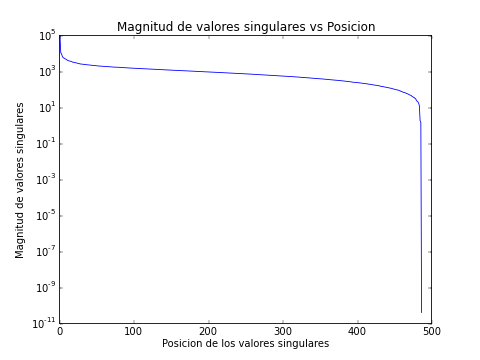
\includegraphics[width=90mm]{./Graficos/fractal-svalue}
			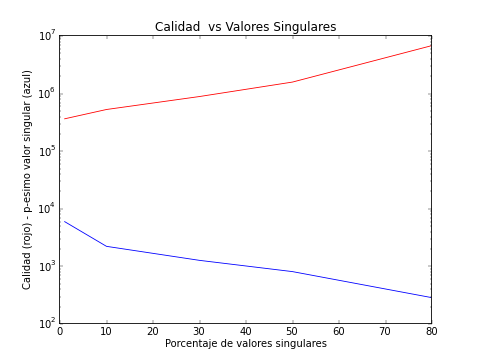
\includegraphics[width=90mm]{./Graficos/fractal-quality}
			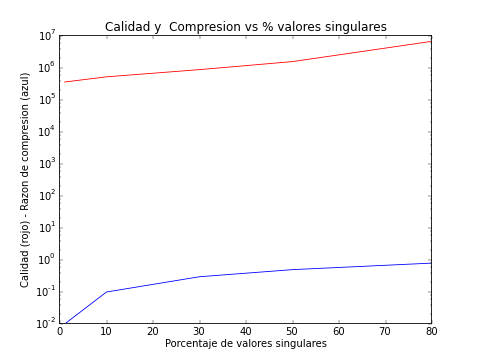
\includegraphics[width=90mm]{./Graficos/fractal-size}
			\label{fig:figura1}
		\end{minipage}%
		\begin{minipage}[b]{0.5\linewidth}
			\caption{Gráficos para paisaje.png}
			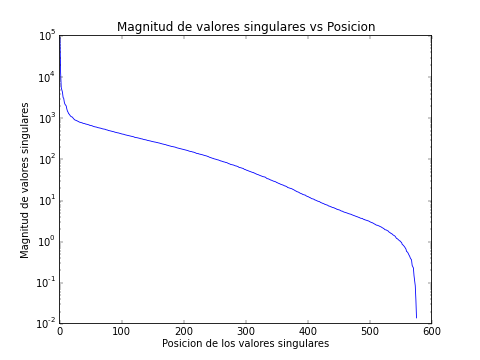
\includegraphics[width=90mm]{./Graficos/paisaje-svalue}
			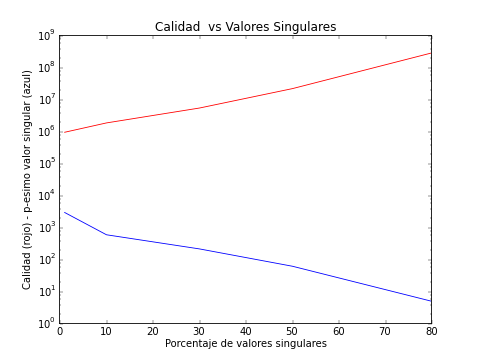
\includegraphics[width=90mm]{./Graficos/paisaje-quality}
			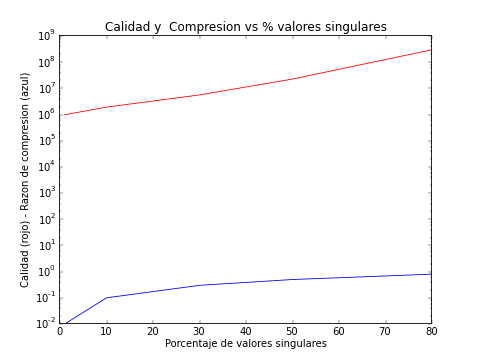
\includegraphics[width=90mm]{./Graficos/paisaje-size}
			\label{fig:figura2}
		\end{minipage}
	\end{figure}

	\begin{figure}[htbp]
		\begin{minipage}[b]{0.5\linewidth}
			\caption{Gráficos para logo-di.bmp}
			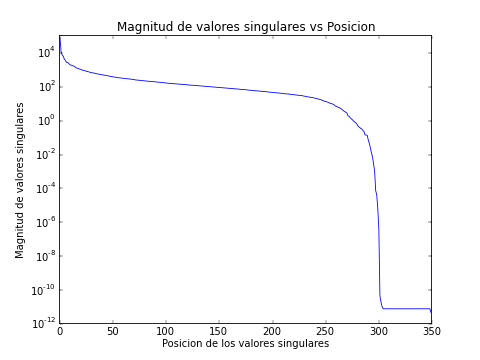
\includegraphics[width=90mm]{./Graficos/logo-di-svalue}
			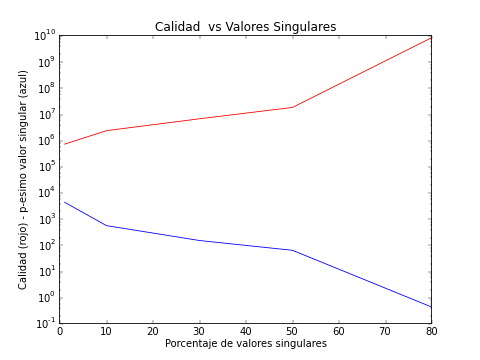
\includegraphics[width=90mm]{./Graficos/logo-di-quality}
			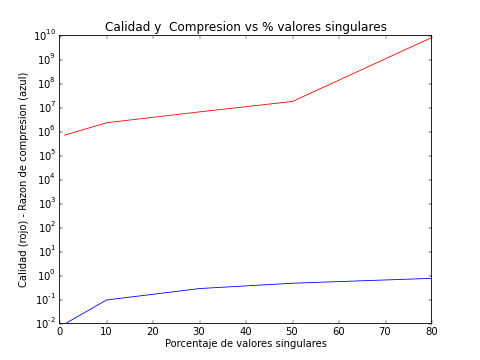
\includegraphics[width=90mm]{./Graficos/logo-di-size}
			\label{fig:figura3}
		\end{minipage}%
		\begin{minipage}[b]{0.5\linewidth}
			\caption{Gráficos para matriz1.txt}
			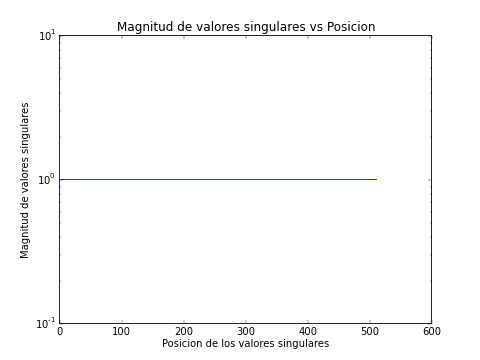
\includegraphics[width=90mm]{./Graficos/matriz1-svalue}
			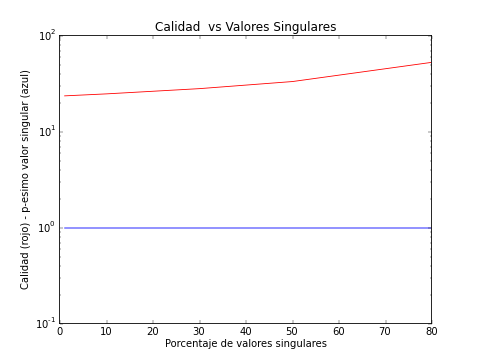
\includegraphics[width=90mm]{./Graficos/matriz1-quality}
			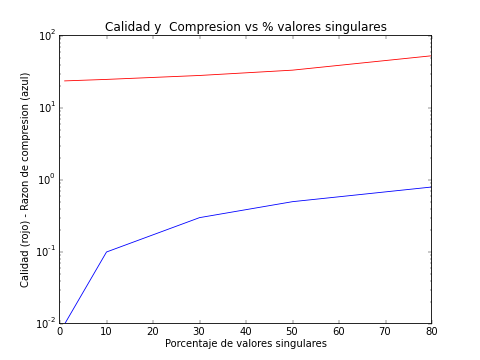
\includegraphics[width=90mm]{./Graficos/matriz1-size}
			\label{fig:figura4}
		\end{minipage}
	\end{figure}

	\begin{figure}[htbp]
		\begin{minipage}[b]{0.5\linewidth}
			\caption{Gráficos para matriz2.txt}
			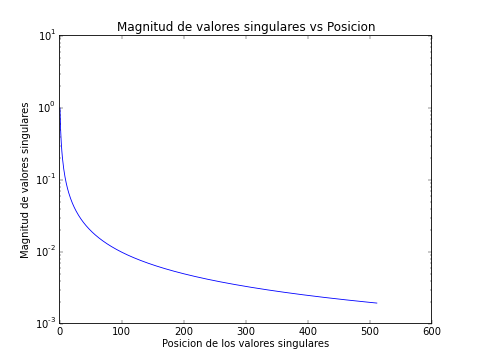
\includegraphics[width=90mm]{./Graficos/matriz2-svalue}
			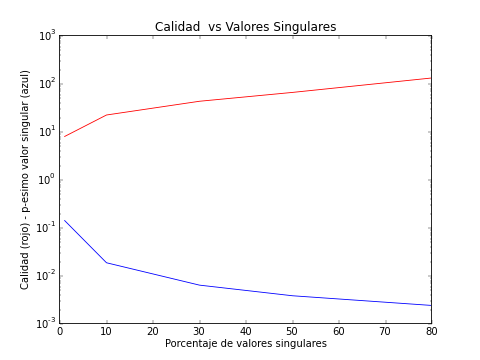
\includegraphics[width=90mm]{./Graficos/matriz2-quality}
			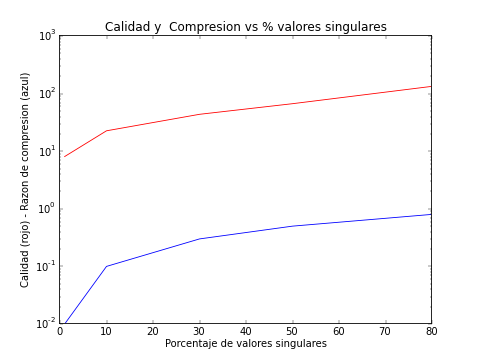
\includegraphics[width=90mm]{./Graficos/matriz2-size}
			\label{fig:figura5}
		\end{minipage}%
		\begin{minipage}[b]{0.5\linewidth}
			\caption{Gráficos para matriz3.txt}
			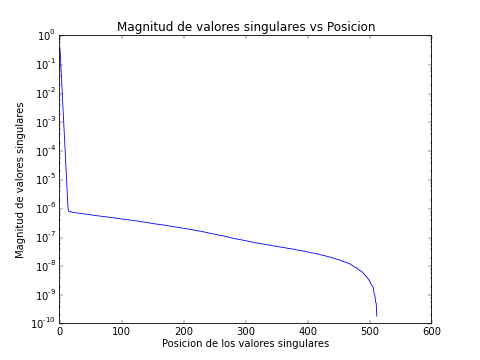
\includegraphics[width=90mm]{./Graficos/matriz3-svalue}
			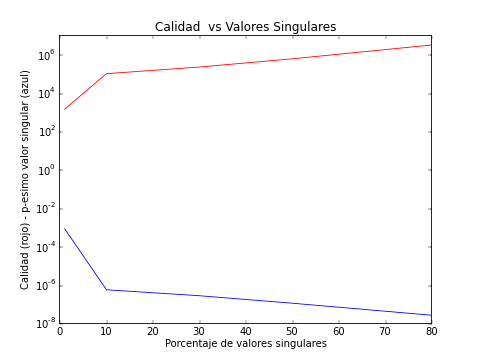
\includegraphics[width=90mm]{./Graficos/matriz3-quality}
			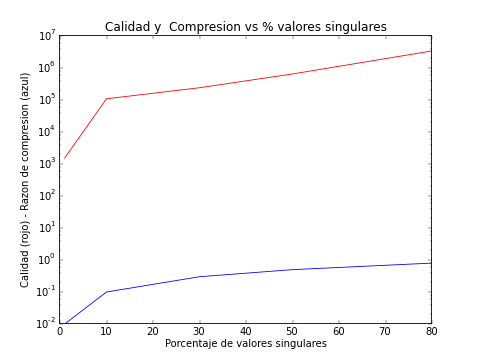
\includegraphics[width=90mm]{./Graficos/matriz3-size}
			\label{fig:figura6}
		\end{minipage}
	\end{figure}

	\begin{figure}[htbp]
		\begin{minipage}[b]{0.5\linewidth}
			\caption{Gráficos para matriz4.txt}
			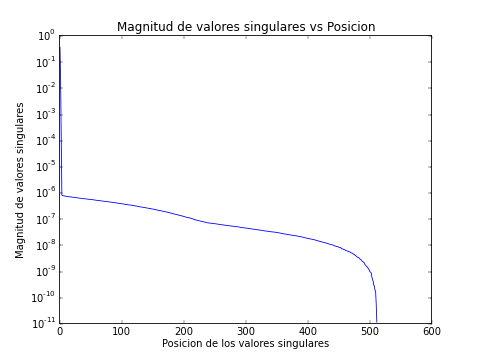
\includegraphics[width=90mm]{./Graficos/matriz4-svalue}
			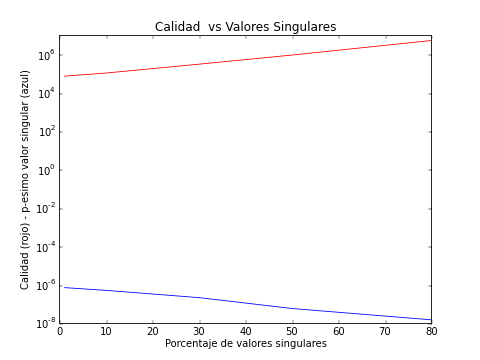
\includegraphics[width=90mm]{./Graficos/matriz4-quality}
			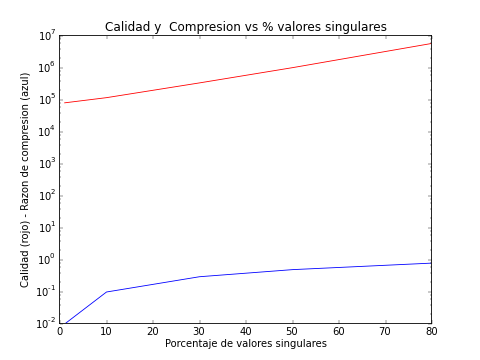
\includegraphics[width=90mm]{./Graficos/matriz4-size}
			\label{fig:figura7}
		\end{minipage}%
		\begin{minipage}[b]{0.5\linewidth}
			\caption{Gráficos para matriz5.txt}
			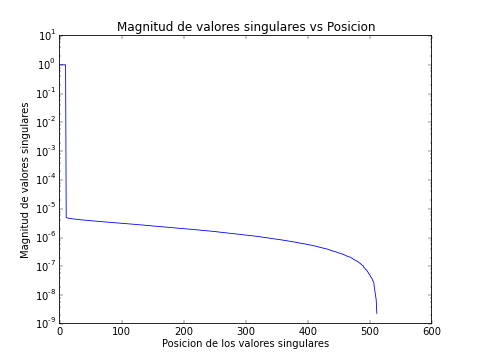
\includegraphics[width=90mm]{./Graficos/matriz5-svalue}
			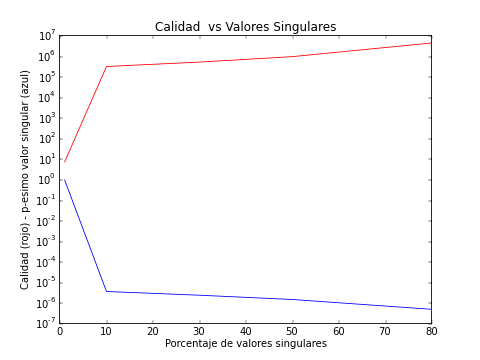
\includegraphics[width=90mm]{./Graficos/matriz5-quality}
			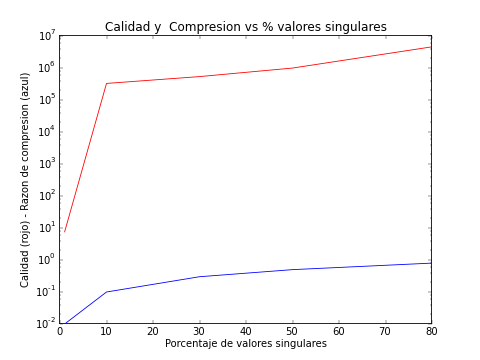
\includegraphics[width=90mm]{./Graficos/matriz5-size}
			\label{fig:figura8}
		\end{minipage}
	\end{figure}
\section{Conclusiones}
	%Conclusiones
	Hemos logrado analizar varios casos de compresión de imágenes por medio de
	la factorización SVD, ésto nos permite comprimir la imagen para que ocupe
	un menor espacio en el disco duro, pero por ello debemos pagar el precio
	en la calidad de dicha imagen. En general, notamos que con un margen de
	compresión del $10\%$, la perdida de calidad es lo suficientemente pequeña
	como para ser aceptable.\\
	Gracias a los gráficos de las matrices generadas por los ficheros de texto,
	podemos ver casos especiales en los cuales los valores singulares se
	comportan de manera tal que se hace posible una compresión muy mayor a lo
	que sucede normalmente, pero creemos que no es muy común en la generalidad
	de las imágenes.\\
	Como vimos en los gráficos, la compresión puede disminuir notablemente el
	tamaño de las imágenes, pero esto solo se notará si disponemos de los medios
	necesarios para guardar dicho archivo como su descomposición y no como una
	matriz, lo que implicaría un proceso de visualización más complejo.

\newpage
\section{Anexo}
	%hack para acentos:
	\lstset{literate=
		{á}{{\'a}}1 {é}{{\'e}}1 {í}{{\'i}}1 {ó}{{\'o}}1 {ú}{{\'u}}1
		{Á}{{\'A}}1 {É}{{\'E}}1 {Í}{{\'I}}1 {Ó}{{\'O}}1 {Ú}{{\'U}}1
		{à}{{\`a}}1 {è}{{\'e}}1 {ì}{{\`i}}1 {ò}{{\`o}}1 {ù}{{\`u}}1
		{À}{{\`A}}1 {È}{{\'E}}1 {Ì}{{\`I}}1 {Ò}{{\`O}}1 {Ù}{{\`U}}1
		{ä}{{\"a}}1 {ë}{{\"e}}1 {ï}{{\"i}}1 {ö}{{\"o}}1 {ü}{{\"u}}1
		{Ä}{{\"A}}1 {Ë}{{\"E}}1 {Ï}{{\"I}}1 {Ö}{{\"O}}1 {Ü}{{\"U}}1
		{â}{{\^a}}1 {ê}{{\^e}}1 {î}{{\^i}}1 {ô}{{\^o}}1 {û}{{\^u}}1
		{Â}{{\^A}}1 {Ê}{{\^E}}1 {Î}{{\^I}}1 {Ô}{{\^O}}1 {Û}{{\^U}}1
		{œ}{{\oe}}1 {Œ}{{\OE}}1 {æ}{{\ae}}1 {Æ}{{\AE}}1 {ß}{{\ss}}1
		{ç}{{\c c}}1 {Ç}{{\c C}}1 {ø}{{\o}}1 {å}{{\r a}}1 {Å}{{\r A}}1
		{€}{{\EUR}}1 {£}{{\pounds}}1 {ñ}{{\~n}}1
	}

%Anexo con código utilizado
	\lstinputlisting[language=Python,
				 frame=single,
				 showstringspaces=false,
				 commentstyle=\color{gris},
				 title=\lstname,
			 	 tabsize=4]{../Codigos/Laboratorio3.py}

\vfill\hfill HV/AS/\LaTeXe
\end{document}
